\documentclass{article}
\usepackage[utf8]{inputenc}
\usepackage{amsfonts,latexsym,amsthm,amssymb,amsmath,amscd,euscript}
\usepackage{float}
\usepackage{graphicx}
\usepackage{mathtools}
\usepackage{framed}

\usepackage{listings}
\usepackage{color} %red, green, blue, yellow, cyan, magenta, black, white

\usepackage{verbatim}

\definecolor{mygreen}{RGB}{28,172,0} % color values Red, Green, Blue
\definecolor{mylilas}{RGB}{170,55,241}
% Descomentar fullpage cuando se quiera utilizar menos margen horizontal
%\usepackage{fullpage}
\usepackage{hyperref}
    \hypersetup{colorlinks=true,citecolor=blue,urlcolor =black,linkbordercolor={1 0 0}}

\newenvironment{statement}[1]{\smallskip\noindent\color[rgb]{1.00,0.00,0.50} {\bf #1.}}{}
\allowdisplaybreaks[1]

% Comandos para teoremas, definiciones, ejemplos, lemas, etc. para sus respectivos body types.
\renewcommand*{\proofname}{Prueba}
\renewcommand{\contentsname}{Contenido}

\newtheorem{theorem}{Teorema}
\newtheorem*{proposition}{Proposici\'on}
\newtheorem{lemma}[theorem]{Lema}
\newtheorem{corollary}[theorem]{Corolario}
\newtheorem{conjecture}[theorem]{Conjetura}
\newtheorem*{postulate}{Postulado}
\theoremstyle{definition}
\newtheorem{defn}[theorem]{Definici\'on}
\newtheorem{example}[theorem]{Ejemplo}

\theoremstyle{remark}
\newtheorem*{remark}{Observaci\'on}
\newtheorem*{notation}{Notaci\'on}
\newtheorem*{note}{Nota}
\newtheorem*{solution}{Soluci\'on}

% Define tus comandos para hacer la vida más fácil.
\newcommand{\BR}{\mathbb R}
\newcommand{\BC}{\mathbb C}
\newcommand{\BF}{\mathbb F}
\newcommand{\BQ}{\mathbb Q}
\newcommand{\BZ}{\mathbb Z}
\newcommand{\BN}{\mathbb N}

% MATLAB
\lstset{language=Matlab,%
  %basicstyle=\color{red},
  breaklines=true,%
  morekeywords={matlab2tikz},
  keywordstyle=\color{blue},%
  morekeywords=[2]{1}, keywordstyle=[2]{\color{black}},
  identifierstyle=\color{black},%
  stringstyle=\color{mylilas},
  commentstyle=\color{mygreen},%
  showstringspaces=false,%without this there will be a symbol in the places where there is a space
  numbers=left,%
  numberstyle={\tiny \color{black}},% size of the numbers
  numbersep=9pt, % this defines how far the numbers are from the text
  emph=[1]{for,end,break},emphstyle=[1]\color{red}, %some words to emphasise
  %emph=[2]{word1,word2}, emphstyle=[2]{style},
}

% Inicio del documento

\title{MAT237 C\'alculo Num\'erico}
\author{Manuel Loaiza Vasquez}
\date{Septiembre 2021}

\begin{document}

\maketitle

\vspace*{-0.25in}
\centerline{Pontificia Universidad Cat\'olica del Per\'u}
\centerline{Lima, Per\'u}
\centerline{\href{mailto:manuel.loaiza@pucp.edu.pe}{{\tt manuel.loaiza@pucp.edu.pe}}}
\vspace*{0.15in}

\begin{framed}
  Solucionario de la Pr\'actica Calificada 1 del curso C\'alculo Num\'erico
  de la especialidad de Matem\'aticas de la Facultad de Ciencias e Ingenier\'ia
  dictado por el profesor Rub\'en Agapito durante el ciclo $2021-2$.
\end{framed}

\begin{statement}{1}
  Use la regla de la cadena para obtener los n\'umeros de condicionamiento de
  las siguientes funciones:
\end{statement}

\begin{statement}{a}
  $f(x) = \cos(2 \pi x)$
\end{statement}

\begin{solution}
  Primero probemos el siguiente lema:

  \begin{lemma}
    \label{lemma01}
    Sean $f:\BR \to \BR$ y $g:\BR \to \BR$ funciones continuas diferenciables y
    $h: \BR \to \BR$ con $h(x) = f(g(x))$, luego
    \[
      \kappa_h(x) = \kappa_f(g(x)) \cdot \kappa_g(x).
    \]
  \end{lemma}

  \begin{proof}
    Aplicamos la f\'ormula de condicionamiento a $h$ y la regla de la cadena
    \begin{align*}
      \kappa_h(x) &= \left|x \cdot \frac{h'(x)}{h(x)}\right|\\
      &= \left|x \cdot \frac{f'(g(x)) g'(x)}{f(g(x))}\right|\\
      &= \left|g(x) \cdot \frac{f'(g(x))}{f(g(x))}\right| \cdot \left|x \cdot \frac{g'(x)}{g(x)}\right|\\
      &= \kappa_f(g(x)) \cdot \kappa_g(x).
    \end{align*}
    obteniendo la expresi\'on buscada.
  \end{proof}

  Sean $g: \BR \to \BR$ y $h: \BR \to \BR$ con $g(x) = cos(x)$ y $h(x) = 2 \pi x$.
  Tenemos que $f = g \circ h$, por lo que
  \begin{align*}
    \kappa_f(x) &= \kappa_g(h(x)) \cdot \kappa_h(x)\\
    &= \left|2 \pi x \cdot \frac{-\sin(2 \pi x)}{\cos(2 \pi x)}\right| \cdot \left|x \cdot \frac{2 \pi}{2 \pi x}\right|\\
    &= 2\pi|x \tan(2 \pi x)|.
  \end{align*}
\end{solution}

\begin{statement}{b}
  $f(x) = e^{-x^2}$
\end{statement}

\begin{solution}
  Sean $g: \BR \to \BR$ y $h: \BR \to \BR$ con $g(x) = e^x$ y $h(x) = -x^2$.
  Tenemos que $f = g \circ h$, por lo que
  \begin{align*}
    \kappa_f(x) &= \kappa_g(h(x)) \cdot \kappa_h(x) \\
    &= \left|-x^2 \cdot \frac{e^{-x^2}}{e^{-x^2}}\right|\cdot 2 \\
    &= 2x^2.
  \end{align*}
\end{solution}

\begin{statement}{2}
  Suponga que $f$ es una funci\'on con n\'umero de condicionamiento
  $\kappa_f$ y que $f^{-1}$ es su funci\'on inversa. Demuestre que el n\'umero
  de condicionamiento de $f^{-1}$ satisface
  \[
    \kappa_{f^{-1}(x)} = \frac{1}{\kappa_f(f^{-1}(x))}
  \]
  provisto que el denominador es diferente de cero.
\end{statement}

\begin{proof}
  Analicemos el producto $\kappa_f(f^{-1}(x)) \cdot \kappa_{f^{-1}}(x)$.
  De acuerdo a Lema \ref{lemma01}
  \[
    \kappa_f(f^{-1}(x)) \cdot \kappa_{f^{-1}}(x) = \kappa_{f \circ f^{-1}(x)}(x) = \kappa_x(x) = 1.
  \]
  Ya que nos garantizan que la expresi\'on de la izquierda es distinta de cero,
  pasamos a dividir esta y concluimos con la prueba obteniendo lo requerido.
\end{proof}

\begin{statement}{3}
  El polinomio $x^2 - 2x + 1$ tiene una ra\'iz doble en $r = 1$.
\end{statement}

\begin{statement}{a}
  Use MATLAB para hacer una tabla de las ra\'ices de
  \[
    x^2 - (2 + \varepsilon)x + 1,  
  \]
  para $\varepsilon = 10^{-n}$ con $n = 4, 6, \dots, 12$.
\end{statement}

\begin{solution}
  Utilicemos el siguiente script en MATLAB y el comando \texttt{fzero}

  \lstinputlisting{scripts/ex_03.m}

  para obtener la tabla de ra\'ices
  \begin{center}
    \texttt{Roots of the polynomial $x^2$ - (2 + eps) x + 1}\\
    \texttt{eps = 1.000000e-04, root = 0.9900498750}\\
    \texttt{eps = 1.000000e-06, root = 0.9990004999}\\
    \texttt{eps = 1.000000e-08, root = 0.9999000050}\\
    \texttt{eps = 1.000000e-10, root = 0.9999900001}\\
    \texttt{eps = 1.000000e-12, root = 0.9999989999}
  \end{center}
\end{solution}

\begin{statement}{b}
  ¿Qu\'e puede inferir de los resultados del inciso (a) sobre el n\'umero de
  condicionamiento de la ra\'iz?
\end{statement}

\begin{solution}
  Consideremos el problema de hallar las ra\'ices de $at^2 + bt + c$ cuando
  solo $b$ var\'ia y $a$ y $c$ son constantes. Derivamos impl\'icitamente con
  respecto a $b$:
  \begin{align*}
    \frac{d}{db} (at^2 + bt + c) &= 0\\
    2at\frac{dt}{db} + t + b \frac{dt}{db} &= 0\\
    \frac{dt}{db}(2at + b) &= -t\\
    \frac{dt}{db} &= \frac{-t}{2at + b}.
  \end{align*}
  Ahora calculamos
  \[
    \kappa_t(b) = \left|b \cdot \frac{dt / db}{t}\right| = \left|\frac{b}{\sqrt{b^2 - 4ac}}\right|
    = \left|\frac{b}{a (t_1 - t_2)}\right|
  \]
\end{solution}

\begin{statement}{4}
  Use el m\'etodo de bisecci\'on para encontrar dos n\'umeros reales $x$, con
  seis cifras de exactitud, que hagan que el determinante de la matriz
  \[
    A = \begin{pmatrix}
      1 & 2 & 3 & x \\
      4 & 5 & x & 6 \\
      7 & x & 8 & 9 \\
      x & 10 & 11 & 12
    \end{pmatrix}  
  \]
  sea igual a $1000$. Para cada soluci\'on, calcule el determinante
  correspondiente y reporte cu\'antos decimales correctos (despu\'es del punto
  decimal) tiene el determinante cuando su soluci\'on $x$ es usada.
\end{statement}

\begin{solution}
  Primero, necesitamos definir una funci\'on objetivo $f: \BR \to \BR$ con
  \[
    f(x) = \det(A(x)) - 1000
  \]
  reduciendo as\'i nuestro problema a hallar las ra\'ices de esta.
  Esbocemos $f$ en el intervalo $[-20, 20)$ para poder hacernos una idea de en
  qu\'e intervalos la funci\'on es mon\'otona y tiene ra\'ices para poder aplicar
  b\'usqueda binaria.

  \begin{figure}[H]
    \centering
    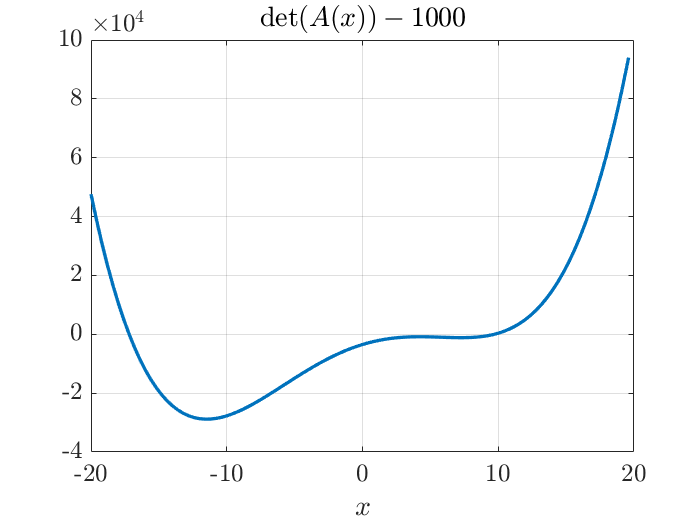
\includegraphics[scale=0.5]{graphics/plot.png}
    \caption{Esbozo de $f$}
  \end{figure}

  De la gr\'afica observamos que una ra\'iz se encuentra en el intervalo
  $[-20, -15]$ y la otra en el intervalo $[9, 10]$.
  \begin{itemize}
    \item Aplicamos b\'usqueda binaria en el intervalo $[-20, -15]$, obteniendo la
    ra\'iz aproximada $-17.188498$. Evaluamos $f(-17.188498) = -0.000853$,cuyo
    valor absoluto al compararse con cero tiene tres decimales correctos.
    \item Aplicamos b\'usqueda binaria en el intervalo $[9, 10]$, obteniendo la
    ra\'iz aproximada $9.708299$. Evaluamos $f(9.708299) = -0.000230$,cuyo
    valor absoluto al compararse con cero tiene tres decimales correctos.
  \end{itemize}
\end{solution}

\lstinputlisting{scripts/ex_04.m}

\begin{statement}{5}
  Encuentre tres formas diferentes $g(x)$ para encontrar ra\'ices con seis
  cifras de exactitud de $f(x) = 0$ por el m\'etodo de iteraci\'on de punto fijo.
  Cada ecuaci\'on $f(x) = 0$ tiene tres ra\'ices. Encuentre m\'as $g(x)$ si fuese
  necesario hasta que todas las ra\'ices sean encontradas por el m\'etodo.
  Para cada iteraci\'on convergente, estime el valor de $|g'(r)|$ en base a
  los errores $e_{k + 1} / e_k$ y comp\'arelo con el valor $|g'(r)|$, donde $r$
  es la ra\'iz aproximada obtenida y $g'(x)$ es calculada anal\'iticamente.
\end{statement}

\begin{statement}{a}
  $f(x) = 2x^3 - 6x - 1$
\end{statement}

\begin{solution}
  Utilicemos el siguiente script en MATLAB para hallar las tres ra\'ices aproximadas
  de $f$ utilizando el m\'etodo de iteraci\'on de punto fijo
  \lstinputlisting{scripts/ex_05_01.m}
  obteniendo como salida

  \verbatiminput{outputs/ex_05_01.txt}

  Ahora analicemos anal\'iticamente cada una de las funciones $g$:
  \begin{itemize}
    \item $g(x) = (2x^3 - 1) / 6$. Tenemos $g'(x) = x^2$, por lo que
    \[
      |g'(-0.168254)| \approx 0.028309408516 < 1
    \]
    el MIPF converge localmente.
    \item $g(x) = ((6x + 1) / 2)^{1 / 3}$. Tenemos $g'(x) = 1 / (3x + 1/2)^{2 / 3}$, por lo que
    \[
      |g'(1.810039)| \approx 0.305228 < 1  
    \]
    el MIPF converge localmente.
    \item $g(x) = (4x^3 + 1) / (6x^2 - 6)$. Tenemos $g'(x) = (x (2x^3 - 6x - 1)) / (2(x^2 - 1)^2)$, por lo que
    \[
      |g'(-1.641784)| \approx 9.15176 \times 10^{-7}< 1
    \]
    el MIPF converge localmente.
  \end{itemize}
\end{solution}

\begin{statement}{b}
  $f(x) = e^{x - 2} + x^3 - x$
\end{statement}

\begin{solution}
  Utilicemos el siguiente script en MATLAB para hallar las tres ra\'ices aproximadas
  de $f$ utilizando el m\'etodo de iteraci\'on de punto fijo
  \lstinputlisting{scripts/ex_05_02.m}
  obteniendo como salida

  \verbatiminput{outputs/ex_05_02.txt}

  Ahora analicemos anal\'iticamente cada una de las funciones $g$:
  \begin{itemize}
    \item $g(x) = e^{x - 2} + x^3$. Tenemos $g'(x) = e^{x - 2} + 3x^2$, por lo que
    \[
      |g'(0.163822)| \approx 0.239939 < 1
    \]
    el MIPF converge localmente.
    \item $g(x) = (x - e^{x - 2})^{1 / 3}$. Tenemos $g'(x) = (1 - e^{x - 2}) / (3(x - e^{x - 2})^{2 / 3})$, por lo que
    \[
      |g'(0.788940)| \approx 0.376011 < 1
    \]
    el MIPF converge localmente.
    \item $g(x) = (-e^{x - 2} + 2x^3) / (3x^2 - 1)$. Tenemos
    \[
      g'(x) = \frac{6x^2 - e^{x - 2}}{3x^2 - 1} - \frac{6x(2x^3 - e^{x - 2})}{(3x^2 - 1)^2},
    \]
    por lo que
    \[
      |g'(-1.023482)| \approx 0.0226986 < 1
    \]
    el MIPF converge localmente.
  \end{itemize}
\end{solution}

\end{document}

